% 7:10
% -50

\begin{solutionbox}[Q1-1]
    \begin{center}
        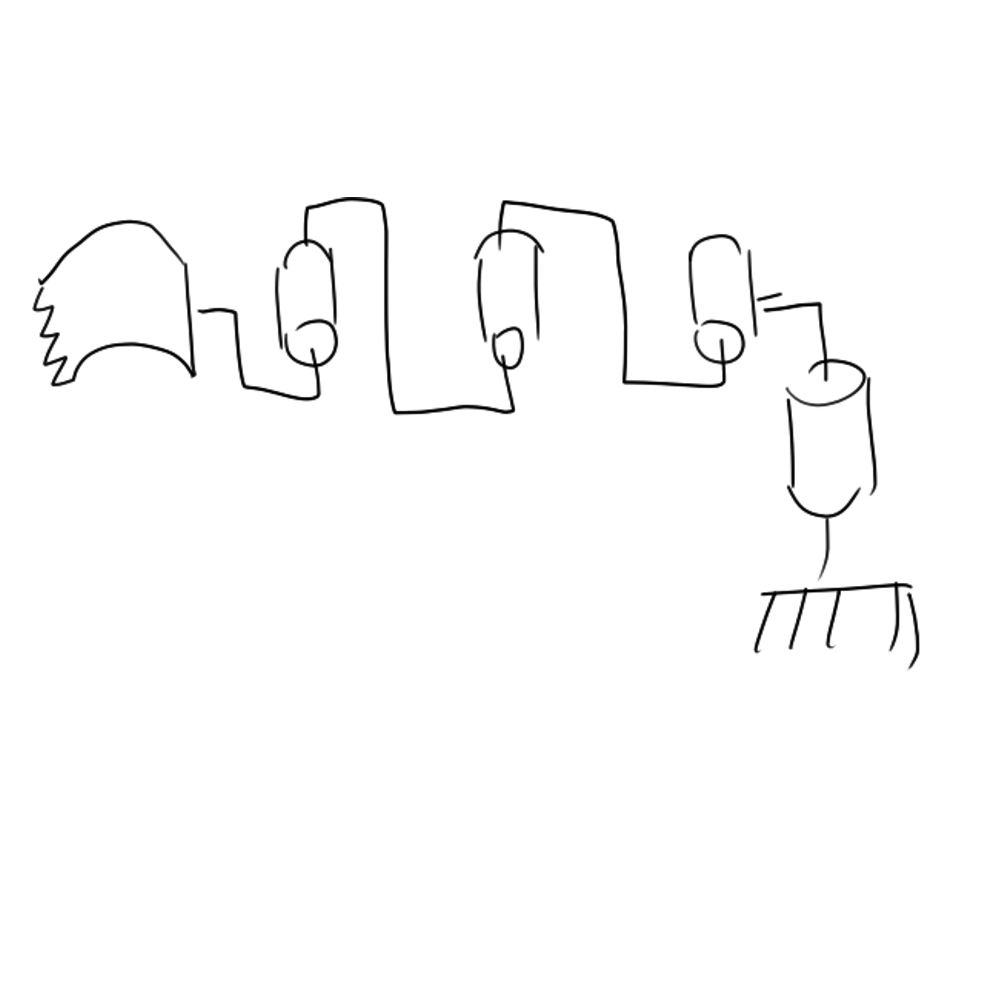
\includegraphics[width=120mm]{imgs/y2024-v1-q1-1.png}
    \end{center}
\end{solutionbox}


\begin{solutionbox}[Q1-2]
    \begin{align*}
        {\,^5\omega_{6,5}}      & = \dot{\theta_6} k                                                                                       \\
        {\pv{\omega}_{6,5}}     & = \pc{C}_5 \dot{\theta_6} k                                                                              \\
        {\pv{\omega}_{6,5}}     & = \pc{C}_4 e^{\theta_5 k\times}e^{-\psi i\times} \dot{\theta_6} k                                        \\
        {\pv{\omega}_{6,5}}     & = \pc{C}_3 e^{\theta_4 k\times} e^{\psi i \times} e^{\theta_5 k\times}e^{-\psi i\times} \dot{\theta_6} k \\
        {\,^3\pv{\omega}_{6,5}} & =e^{\theta_4 k\times} e^{\psi i \times} e^{\theta_5 k\times}e^{-\psi i\times} \dot{\theta_6} k           \\
    \end{align*}

    \begin{align*}
        {\,^4\omega_{5,4}}      & = \dot{\theta_5} k                                                 \\
        {\pv{\omega}_{5,4}}     & = \pc{C}_4 \dot{\theta_5} k                                        \\
        {\pv{\omega}_{5,4}}     & = \pc{C}_3 e^{\theta_4 k\times} e^{\psi i \times} \dot{\theta_5} k \\
        {\,^3\pv{\omega}_{5,4}} & =e^{\theta_4 k\times} e^{\psi i \times} \dot{\theta_5} k           \\
    \end{align*}
    \begin{align*}
        {\,^3\omega_{4,3}} & = \dot{\theta_3} k \\
    \end{align*}

    \begin{align*}
        {\,^3\omega_{6,3}} & ={\,^3\omega_{6,5}}  + {\,^3\omega_{5,4}}  + {\,^3\omega_{4,3}}                                                                           \\
        {\,^3\omega_{6,3}} & =  \dot{\theta_3} k + e^{\theta_4 k\times} e^{\psi i \times} ( \dot{\theta_5} k +e^{\theta_5 k\times}e^{-\psi i\times} \dot{\theta_6} k ) \\
    \end{align*}


\end{solutionbox}

\begin{solutionbox}[Q1-3]

    The question is identical to that in Exam 2025.

    I think there is still value so i redid it with different working.

    First find the direction to move the end effector to move from $\ppori{a}$ to $\ppori{b}$ which is $(\ppori{b}-\ppori{a})$.

    Second find the axis and angle to rotate such that the effector rotates from $\pc{C}_a$ to $\pc{C}_b$.

    Third, decide the profile to move by. This is the step where quintic polynomial comes in as it is the minimum number of degrees such that the initial and final position, velocity, and acceleration can be independently set.

    Forth, at every time step, compute the inverse kinematics from for the position and orientation at that time stamps.

    The first three steps can be written as the following.
    \begin{align*}
        \ppori{t} = \ppori{a} + s(t) (\ppori{b}-\ppori{a}) \\
        \pc{C}_t = Rot(\pc{C}_a,\hat{u},s(t)\theta)        \\
    \end{align*}
    Where $\pc{C}_b = e^{\theta \hat{u}} \pc{C}_a$, and $s(t)=0$ at $t=0$ and $s(t)=1$ at $t=t_f$.

\end{solutionbox}

\begin{solutionbox}[Q1-4]
    The following should be identical to that in Exam 2025.

    I think there is still value so i redid it.

    \begin{align*}
        T & =\frac{1}{2}M\dot{d_1}^2 + \frac{1}{2}m(\dot{d_1}-l\dot{\theta_2}\sin(\theta_2))^2+\frac{1}{2}m(l\dot{\theta_2}\cos(\theta_2))^2                                              \\
          & =\frac{1}{2}M\dot{d_1}^2 + \frac{1}{2}m\left((\dot{d_1})^2-2l\dot{d_1}\dot{\theta_2}\sin(\theta_2)+(l\dot{\theta_2}\sin(\theta_2))^2+(l\dot{\theta_2}\cos(\theta_2))^2\right) \\
          & =\frac{1}{2}M\dot{d_1}^2 + \frac{1}{2}m\left((\dot{d_1})^2-2l\dot{d_1}\dot{\theta_2}\sin(\theta_2)+(l\dot{\theta_2})^2 \right)                                                \\
          & =\frac{1}{2}(M+m)\dot{d_1}^2 + \frac{1}{2}m\left(-2l\dot{d_1}\dot{\theta_2}\sin(\theta_2)+(l\dot{\theta_2})^2 \right)                                                         \\
        V & =mgl\sin(\theta_2)
    \end{align*}

    \begin{align*}
        L & =T-V                                                                                                                                    \\
          & =\frac{1}{2}(M+m)\dot{d_1}^2 + \frac{1}{2}m\left(-2l\dot{d_1}\dot{\theta_2}\sin(\theta_2)+(l\dot{\theta_2})^2 \right)-mgl\sin(\theta_2) \\
    \end{align*}

    \begin{align*}
        \frac{d}{dt} \left(\frac{\partial L}{\partial \dot{d_1}} \right) - \frac{\partial L}{\partial d_1} & = f_1 \\
        \frac{d}{dt} \left( (M+m)\dot{d_1} -ml\dot{\theta_2}\sin(\theta_2) \right) -0                      & = f_1 \\
        (M+m)\ddot{d_1} -ml\ddot{\theta_2}\sin(\theta_2)-ml\dot{\theta_2}^2\cos(\theta_2)                  & = f_1 \\
    \end{align*}

    \begin{align*}
        \frac{d}{dt} \left(\frac{\partial L}{\partial \dot{\theta_2}} \right) - \frac{\partial L}{\partial \theta_2}                                        & = \tau_2 \\
        \frac{d}{dt} \left(-ml\dot{d_1}\sin(\theta_2)+ml^2\dot{\theta_2} \right) - (-ml\dot{d_1}\dot{\theta_2}\cos(\theta_2)-mgl\cos(\theta_2))             & = \tau_2 \\
        -ml\ddot{d_1}\sin(\theta_2)-ml\dot{d_1}\dot{\theta_2}\cos(\theta_2)+ml^2\ddot{\theta_2} +ml\dot{d_1}\dot{\theta_2}\cos(\theta_2)+ mgl\cos(\theta_2) & = \tau_2 \\
        ml^2\ddot{\theta_2}-ml\ddot{d_1}\sin(\theta_2) + mgl\cos(\theta_2)                                                                                  & = \tau_2 \\
    \end{align*}

\end{solutionbox}

\begin{solutionbox}[Q1-5]
    The following should be identical to that in Exam 2025.

    I think there is still value so i redid it.

    \begin{align*}
        G(q)=
        \begin{bmatrix}
            0 \\
            mgl\cos(\theta_2)
        \end{bmatrix}
    \end{align*}

    \begin{align*}
        D(q) =
        \begin{bmatrix}
            M+m               & -ml\sin(\theta_2) \\
            -ml\sin(\theta_2) & ml^2
        \end{bmatrix}
    \end{align*}

\end{solutionbox}

\begin{solutionbox}[Q1-6]
    The following should be identical to that in Exam 2025.

    I think there is still value so i redid it.

    \begin{align*}
        d_0(t)=0                                                  \\
        \dot{d}_0(t)=0                                            \\
        \ddot{d}_0(t)=0                                           \\
        \theta_0(t)=\frac{-\pi}{2}\cos(\frac{\pi}{T}t)            \\
        \dot{\theta}_0(t)=\frac{\pi^2}{2T}\sin(\frac{\pi}{T}t)    \\\
        \ddot{\theta}_0(t)=\frac{\pi^3}{2T^2}\cos(\frac{\pi}{T}t) \\\
    \end{align*}

    \begin{align*}
        \tau_2 & = ml^2\ddot{\theta_2}-ml\ddot{d_1}\sin(\theta_2) + mgl\cos(\theta_2)                                                 \\
        \tau_2 & = ml^2\left[\frac{\pi^3}{2T^2}\cos(\frac{\pi}{T}t)\right] + mgl\cos(\left[\frac{-\pi}{2}\cos(\frac{\pi}{T}t)\right]) \\
        f_1    & = (M+m)\ddot{d_1} -ml\ddot{\theta_2}\sin(\theta_2)-ml\dot{\theta_2}^2\cos(\theta_2)                                  \\
        f_1    & =
        -ml\left[\frac{\pi^3}{2T^2}\cos(\frac{\pi}{T}t)\right]
        \sin(\left[\frac{-\pi}{2}\cos(\frac{\pi}{T}t)\right])
        -ml\left[\frac{\pi^2}{2T}\sin(\frac{\pi}{T}t)\right]^2
        \cos(\left[\frac{-\pi}{2}\cos(\frac{\pi}{T}t)\right])                                                                         \\
    \end{align*}
\end{solutionbox}

\begin{solutionbox}[Q1-7]
    see Exam 2025 q1-7.
\end{solutionbox}

\begin{solutionbox}[Q1-8]
    see Exam 2025 q1-8.
\end{solutionbox}

\begin{solutionbox}[Q1-9]
    see Exam 2025 q1-9.
\end{solutionbox}